\chapter{Installation and first launch}\label{ch:install}
\index{Installation and Runtime}

KSSOLV Toolbox can run as a standalone application, as a MATLAB\regmark{} toolbox, or in a browser through \ksonline{}. Table~\ref{tab:usage-modes} compares their requirements. This chapter covers standalone installation on Windows, macOS, and Linux, followed by MATLAB\regmark{} toolbox installation and the first launch.

\ksonline{} needs no client installation. Once you have a browser and the service address, follow Chapter~\ref{ch:online} to open a workspace. For a local application or MATLAB\regmark{} toolbox, complete the relevant installation steps below, check the interface, import a small structure, and save a project.

\section{Check the system requirements}

The standalone application uses a matching MATLAB\regmark{} Runtime. It does not require a full MATLAB\regmark{} installation or a MATLAB\regmark{} license. Runtime executes the application; it does not provide the MATLAB\regmark{} desktop programming environment.

The MATLAB\regmark{} toolbox is intended for users with a supported, licensed MATLAB\regmark{} installation. It requires MATLAB\regmark{} R2025a or later; see ``Install the toolbox in MATLAB\regmark{}'' below. If you already have MATLAB\regmark{}, choose the edition according to whether you need workspace variables, scripts, or other MATLAB\regmark{} products.

\subsection{Understand the \headinglatin{Runtime} options}

The standalone application needs the MATLAB\regmark{} Runtime specified for its release. Packages generally provide it in one of three ways: a web installer downloads Runtime when needed, an offline installer includes it, and an application-only installer uses a compatible Runtime already on the computer. The application version identifies KSSOLV Toolbox; the Runtime release identifies its execution environment. These are separate version numbers.

The installer checks for the required Runtime. Even if full MATLAB\regmark{} is installed, follow the detection result to select a matching Runtime or install one.

\begin{notebox}{Choose the right download}
Check the operating system, processor architecture, and package description. Apple silicon and Intel Macs use different application architectures, and Windows and Linux packages are not interchangeable. Follow the filenames and instructions on the release page.
\end{notebox}

\section{Before you install}

Download the installer from the KSSOLV Toolbox release page and put it somewhere easy to find, such as your Downloads folder. Check the release notes for the version, operating system, and processor architecture before choosing a package.

Save your projects and close any older KSSOLV Toolbox instance before installing. Upgrades normally retain projects and personal settings. Keep an internet connection available for a web installation. For an offline package, keep all supplied files in the same directory.

Choose a local disk with enough free space. The application, Runtime, and your projects can be in separate directories: the installer manages the first two, while projects are best kept in a familiar working folder. For example, create a ``Materials calculations'' folder with subfolders for individual materials or projects. This makes your work easier to find than leaving everything in Downloads.

\section{Install on \headinglatin{Windows}}

\subsection{Run the installer}

A Windows standalone distribution is normally a versioned EXE installer with \file{KSSOLV_Toolbox} in its name. Some offline distributions also contain \file{.bin} volume files with the same base name. Keep those files together and run the EXE; do not open the volumes separately.

\begin{steps}
\item Double-click the installer. If User Account Control appears, check the publisher information before allowing it to continue.
\item Choose an installation language and read the instructions. Select English to match this edition of the manual.
\item Read and accept the toolbox and Runtime license terms as prompted, then continue to the application location and Runtime settings.
\item Choose the application directory. Keep the default location or select another local disk.
\item Review the Runtime detection result. Reuse a compatible installation when offered, or choose the Runtime installation method supplied by the package.
\item Start installation and wait for file copying and final configuration to finish. Close the installer after it displays the completion page.
\end{steps}

The application and Runtime can use separate locations, for example:
\begin{itemize}[nosep]
\item Application: \literalinput{E:/Apps/KSSOLV Toolbox}.
\item Runtime: \literalinput{E:/MathWorks/MATLAB Runtime}.
\end{itemize}
The Runtime path must use ASCII characters; letters, digits, and spaces are supported. Project names can describe your research in whichever language you prefer.

\subsection{Wait for installation to finish}

The installer configures the runtime environment near the end of installation. This can take longer when Runtime is being installed for the first time. Wait until the installer reports completion.

If configuration does not finish, follow the retry instructions and check free disk space, directory permissions, and the Runtime source.

The default installation is for all users and normally needs administrator authorization. Per-user installation and reuse of an existing Runtime depend on the options provided by the package. A normal installation does not require changing the system PATH or copying libraries into a MATLAB\regmark{} directory.

\subsection{Launch and update}

After installation, start KSSOLV Toolbox from the Start menu or the shortcut created by the installer. A startup card shows the product name and loading status. When the main window opens, allow the project panels and ribbon to finish loading.

To update, run the new installer and follow its instructions to replace the older application. The installer handles the registered previous version; shared Runtime installations, personal settings, and projects are normally retained. Keep personal projects outside the application installation directory so that program files and research data remain separate during upgrades.

\begin{notebox}{Check offline package files}
If the installer cannot find an additional file, check that the EXE and all matching volume files are together. Also check whether the browser added a duplicate-number suffix to a filename. Confirm that every download is complete, then run the installer again.
\end{notebox}

\section{Install on macOS}

\subsection{Choose the package for your \headinglatin{Mac}}

Open ``About This Mac'' from the Apple menu to check your processor. Apple silicon packages are for Macs with Apple chips. Confirm the architecture before choosing a download.

macOS uses the native Installer to install the PKG. The application normally goes into \file{/Applications}. The installer detects the required Runtime and, depending on the package, reuses, downloads, or installs it. These steps take place in the system installation wizard.

The introduction page lists the application version, processor architecture, and MATLAB\regmark{} Runtime requirements. Check them against your Mac before proceeding. Also check whether the package contains only the application or includes Runtime; the introduction page for your package is the authoritative description.

\begin{steps}
\item Open the downloaded distribution and run its PKG installer.
\item Read the introduction and check the application version, processor architecture, and Runtime release.
\item Read and accept the license terms as prompted, then continue to installation type and location.
\item Select KSSOLV Toolbox and check the application location. The Applications folder is usually appropriate.
\item Review the Runtime settings and choose an existing installation or let the installer prepare one, as described below.
\item Begin installation and authenticate as an administrator when macOS requests it.
\item Wait for the installer to report success, then open KSSOLV Toolbox from Applications.
\end{steps}

Figure~\ref{fig:install-macos-license} shows the license page. Read the terms in the window or use \ui{Print...} or \ui{Save...} to keep a copy. Click \ui{Continue}, then confirm your choice in the agreement dialog. You must agree to proceed with installation. Installation is complete only when the wizard displays its success page.

\screenshot{publication-assets/crop-b9b8c6192e335985ecb0.png}{The license page in the macOS installation wizard. Read the terms in the window, or print or save a copy.}{fig:install-macos-license}

\subsection{Use an existing \headinglatin{Runtime}}

An application-only package requires a compatible Runtime to be installed already. If automatic detection does not find it, select ``Existing MATLAB\regmark{} Runtime'' on the installation type page. Under Location, choose Other and select the release folder requested by the installer. Select the Runtime root directory rather than a library subdirectory within it.

A web installer downloads missing Runtime components from MathWorks; an offline installer uses the supplied files. An existing Runtime can be reused when its release, architecture, and required components match. The installer prepares Runtime before replacing the older toolbox application.

Final configuration takes place in the background and does not necessarily open the Toolbox main window. Wait for the system installer to report success, then launch the application yourself. A startup card on first launch is normal. Later launches still load the runtime environment, but do not repeat installation.

\subsection{Upgrade while retaining projects}

Save your work and close the application before running a new installer. There is no need to move shared Runtime installations, user settings, or projects simply because you are replacing the Toolbox. Keep \file{.ks} files in your Documents folder or a research directory, rather than inside the application bundle.

If macOS asks whether to open an application downloaded from the internet, review the displayed source information before confirming.

\section{Install on \headinglatin{Linux}}

Use the Linux standalone package in a graphical desktop session. If the downloaded installer is already executable, open it from the file manager. Otherwise, open a terminal in the directory containing it.

\begin{steps}
\item Change to the installer directory in a terminal.
\item Make the file executable: \texttt{chmod +x KSSOLV\_Toolbox.install}.
\item Run \texttt{./KSSOLV\_Toolbox.install} to open the graphical installation wizard.
\item Choose the application and Runtime locations, then wait for installation to finish.
\item Launch the application using the entry point or command shown on the completion page.
\end{steps}

The filename above illustrates the usual form; use the actual name of your download. Keep the Runtime path and launch command shown at the end, especially if your desktop environment does not receive an application menu entry automatically.

The Linux standalone application requires a graphical desktop session. To use \ksonline{}, open the Online service in your browser instead.

\section{Install the toolbox in \headinglatin{MATLAB}\regmark{}}

If you have full MATLAB\regmark{}, use \file{KSSOLV_Toolbox.mltbx}. Confirm that MATLAB\regmark{} is R2025a or later, then follow these steps.

\begin{steps}
\item Download \file{KSSOLV_Toolbox.mltbx} from the project release page.
\item Open the file in MATLAB\regmark{} and complete the Add-On installation dialog.
\item Start KSSOLV Toolbox from MATLAB\regmark{} or the Add-On Manager.
\item Wait for the main window before beginning a project exercise.
\end{steps}

If another version is installed, use MATLAB\regmark{}'s Add-On Manager to inspect and manage it. After installation or an upgrade, check that your MATLAB\regmark{} and toolbox versions are compatible before continuing with existing projects.

This manual focuses on the graphical interface. Structure import, modeling, and workflow procedures generally apply to all three editions. Operations involving local files, server-side storage, the MATLAB\regmark{} workspace, or additional MATLAB\regmark{} products are identified where they occur.

\section{Your first launch}

The standalone application first displays a startup card. In Figure~\ref{fig:desktop-startup-050}, the card shows the product version and loading status while the workspace is being prepared. Loading Runtime may take longer on the first launch or after an update. Leave the startup window open and wait for the main window.

\begin{figure}[!htb]
\centering

\includegraphics[width=122mm]{publication-assets/crop-6bf7d3c41caf0892911f.png}
\caption{The KSSOLV Toolbox V0.5.0 standalone startup card, showing the product version and loading status.}
\label{fig:desktop-startup-050}
\end{figure}

Once the startup card closes, the main window shows the Project Browser, ribbon, and central document area. You can then check the version and try a project.

\subsection{Check the interface and version}

Locate the \ui{Home} tab at the top and the \ui{Project Browser} on the left. Choose \ui{Home → Help → About KSSOLV} to check the product version. This manual describes V0.5.0. Select the interface language under \ui{Home → Settings → General}; the change takes effect the next time the application starts.

Figure~\ref{fig:install-workspace-overview} shows an empty project with the main panels expanded. The ribbon provides structure import, workflow creation, and execution controls. The Project Browser lists the project's contents, and the Information Browser below it shows properties of the selected item. The central document area initially displays a welcome message and opens a 3D view when you import a structure. The Config Editor on the right contains parameters, and the Simulation Browser shows run output. The Command Window at the bottom accepts interactive commands; the graphical tutorials do not require you to enter commands there.

\begin{figure}[!htb]
\centering
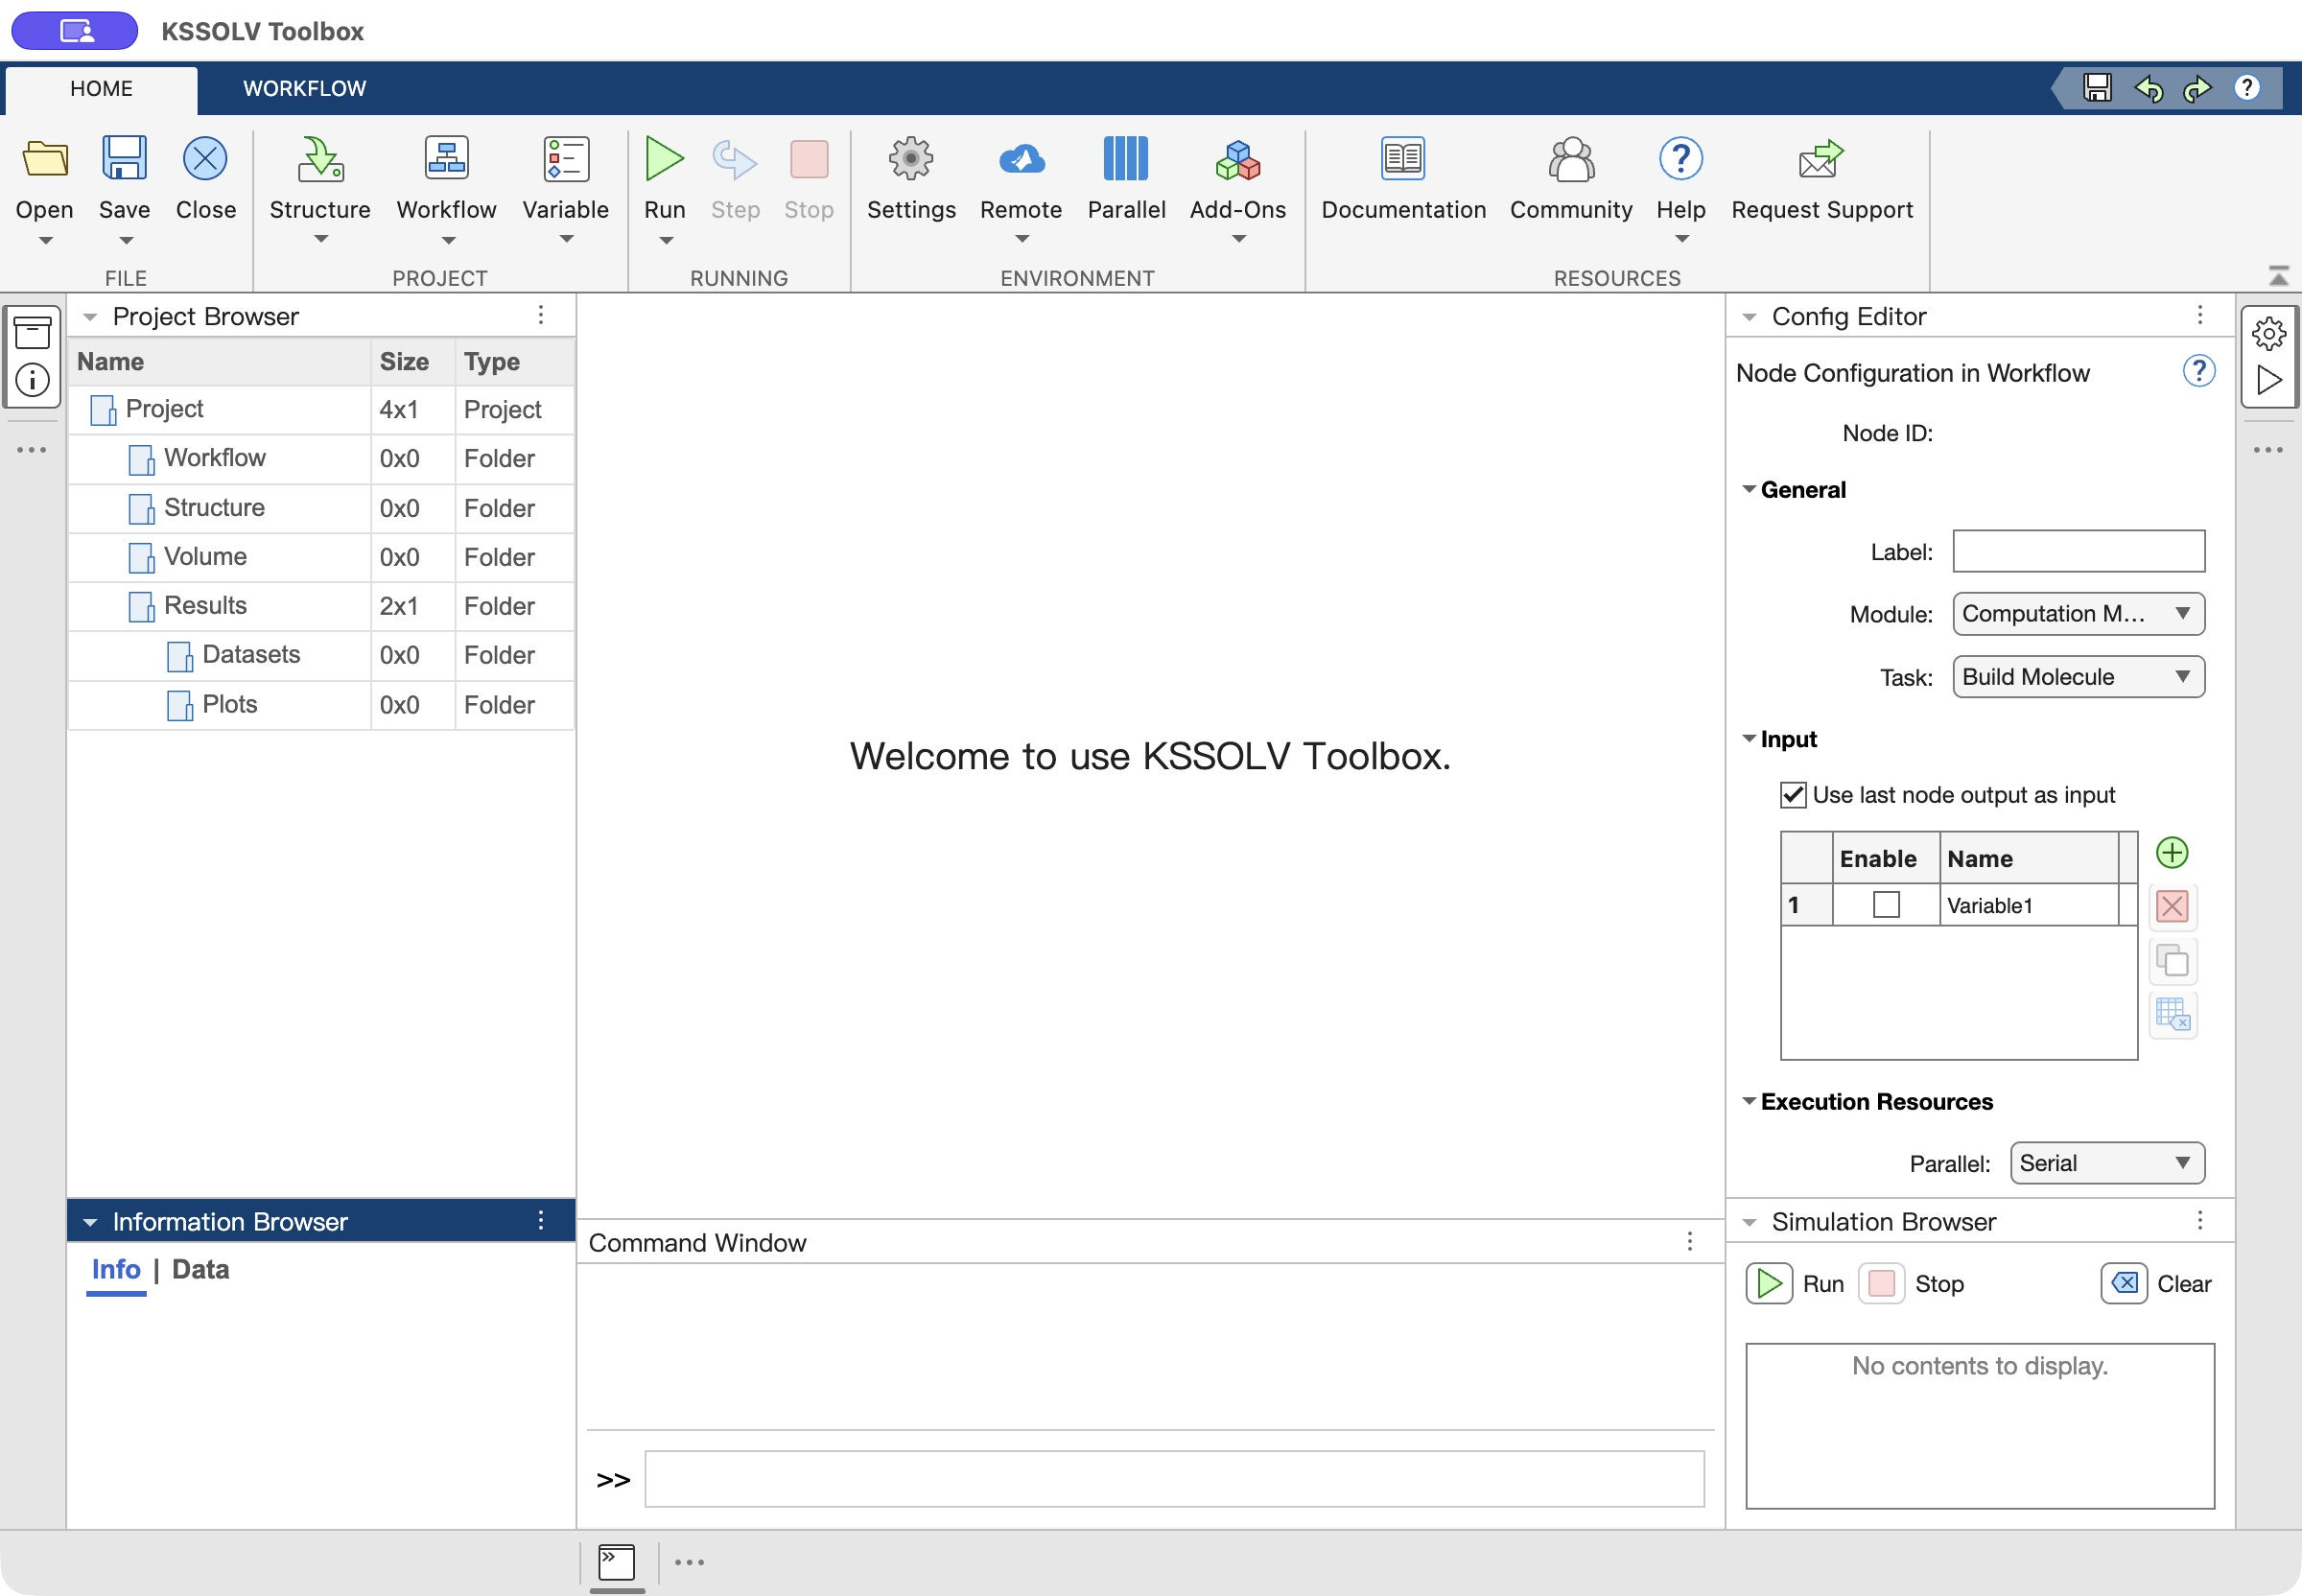
\includegraphics[width=\linewidth]{publication-assets/crop-c885d8ed3b1bcd221501.png}
\caption{The complete desktop workspace. The project, information, configuration, simulation, and command panels are expanded; no structure or workflow document is open yet.}
\label{fig:install-workspace-overview}
\end{figure}

Some panels are collapsed on first launch. Use the button groups at the sides to expand them, or choose a panel from the ellipsis button's \ui{Open Panels} list. The first exercise mainly uses structure import and project saving. Chapter~\ref{ch:workspace} explains each workspace area in detail.

\subsection{Create a project you can reopen}

This exercise checks file handling and the interface without running a calculation. Use the supplied \file{examples/silicon.cif}, or your own small CIF or XYZ file. The supplied silicon structure also provides a direct starting point for the workspace exercise in Chapter~\ref{ch:workspace}.

\begin{steps}
\item Choose \ui{Home → Structure → Import structure from file...} and select the structure file.
\item Check that its name appears in the Project Browser and that atoms appear in the central 3D view.
\item Drag to rotate the view and use the mouse wheel to zoom. Check that the complete structure is visible.
\item Click \ui{Save} and save \file{first-project.ks} in your working directory.
\item Once saving is complete, close the current project and reopen the saved file through \ui{Open Project...}.
\item Check the Project Browser and structure document to confirm that the imported structure is still present.
\end{steps}

You have now checked structure import, 3D display, and project saving. Chapter~\ref{ch:first} takes you through your first electronic structure calculation.

\section{What to check if something goes wrong}

If the application does not start, check that the package matches your processor architecture and that Runtime meets the installer's requirements. When reporting a problem, include the Toolbox version, operating system, installation location, and the complete message shown in the window.

If the main window opens but no 3D structure appears, retry with the small structure used in this chapter and look for a specific graphics message. Online also requires a browser with working WebGL support. If importing a file adds no project item, check the file's format and contents.

If you cannot find a saved file, check where it was saved. The standalone application and MATLAB\regmark{} toolbox use local directories; \ksonline{} uses the server's working directory. Chapter~\ref{ch:online} covers the server-side Files panel and upload and download exercises.

\subsection{Organize files for the next exercises}

Use a consistent project directory. Keep original structures separate from working projects and retain their source information and filenames. Save project copies after structure preparation, parameter checks, and result analysis so that you can return to an earlier stage. When moving work between computers, transfer the complete \file{.ks} project where possible; a structure file alone usually does not contain workflows or calculation results.
